\chapter{Visualizations and Analysis}
\label{chapviz}

When we started out, the initial core data set contained mostly director sharing data. The process of data collection for this dataset is described in data collection section \ref{datacollect}. Interesting insights come about when we dig inside this dataset and try to find out how a big entity is connected to another big entity. \\

Interesting results come about when we merged this dataset with family trees and political data that we obtained. Though this list is a bit long, we have tried to document only the best examples here. \\

We have just been able to touch three realms here: corporate, political, entertainment.
Also, we have tried to see family trees to validate nepotist practices in politics and business. The idea through these visualizations is to show that the power houses interact and mingle mostly among themselves. \\

% 1. sons, daughters, wives, parents, in-lawas share board of director positions
% 2. marraiges in nig power houses among big power houses -- link established explicilty
% 3. business tycoons come baout together to become board of directors
% 4. fmaily trees for corporates large
% 5. politcians and their families linked to croporate realm
% 6. cricketers and their corporate links

\section{Influence Network}

Here we describe the case of politician and business tycoon Naveen Jindal. He is directly on the board of \textbf{8} companies. Through director sharing, in \textbf{2 hops}, he spans \textbf{144} companies, in \textbf{3 hops} the span network is greater than \textbf{1800} companies. Interestingly in \textbf{4 hops}, his influence network reaches more than \textbf{13000 companies out of the 60000 companies} network we have in our DB!  Naveen Jindal is connected to (within 3 hops): \emph{Ashok Leyland, Ambuja cements, Reliance Power, Indiabull, ONGC, JP Associates, Idea, Essar, IDFC, Tata Motors, Shriram, Bharti, Max Life, IDBI, Mahindra, BPCL, Network 18, BHEL, Lanco, Maruti Suzuki, ICICI Bank, Infosys, Adani, ITC, Tech Mahindra, Wipro, HDFC, Hinduja, DLF, Indraprastha Gas, Dabur India, Jet Aiarways, JK Lakshmi Cement} ad nauseum. It is evident as if every big company is connected to the other. Adding to that, he was an MP for ten years.


\begin{figure}[H]
\begin{center}  
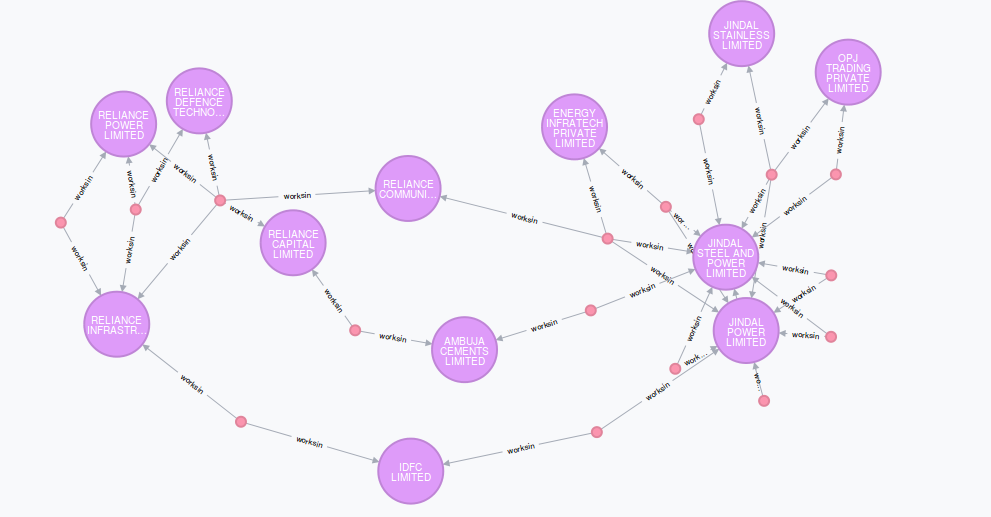
\includegraphics[width=1\textwidth]{nj1} 
\caption{Naveen Jindal's connections with Reliance}
\label{fig:nj1}
\end{center}
\end{figure}

\begin{figure}[H]
\begin{center}  
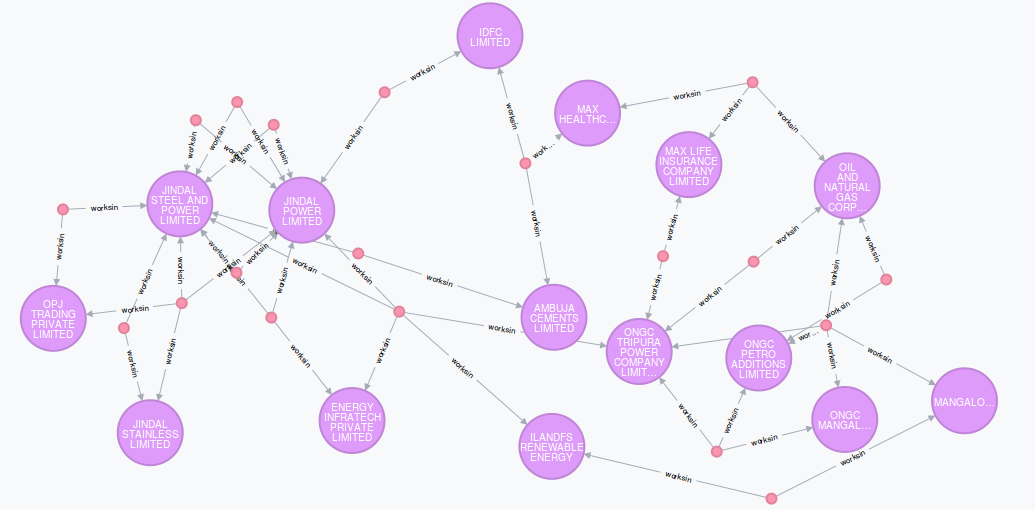
\includegraphics[width=1\textwidth]{nj2} 
\caption{Naveen Jindal's connections with Ambuja Cement and ONGC}
\label{fig:nj2}
\end{center}
\end{figure}


\section{Interesting directors}

\subsection{Not just Mahindra}
\begin{figure}[H]
\begin{center}  
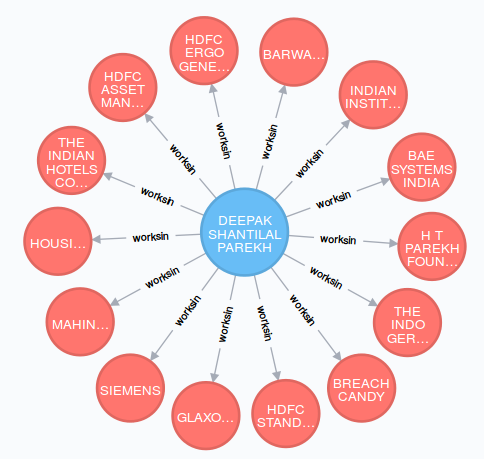
\includegraphics[width=0.4\textwidth]{parekh} 
\caption{Deepak parekh and his first-level directors}
\label{fig:parekh}
\end{center}
\end{figure}


\subsection{The Lavasa Connection}
\begin{figure}[H]
\begin{center}  
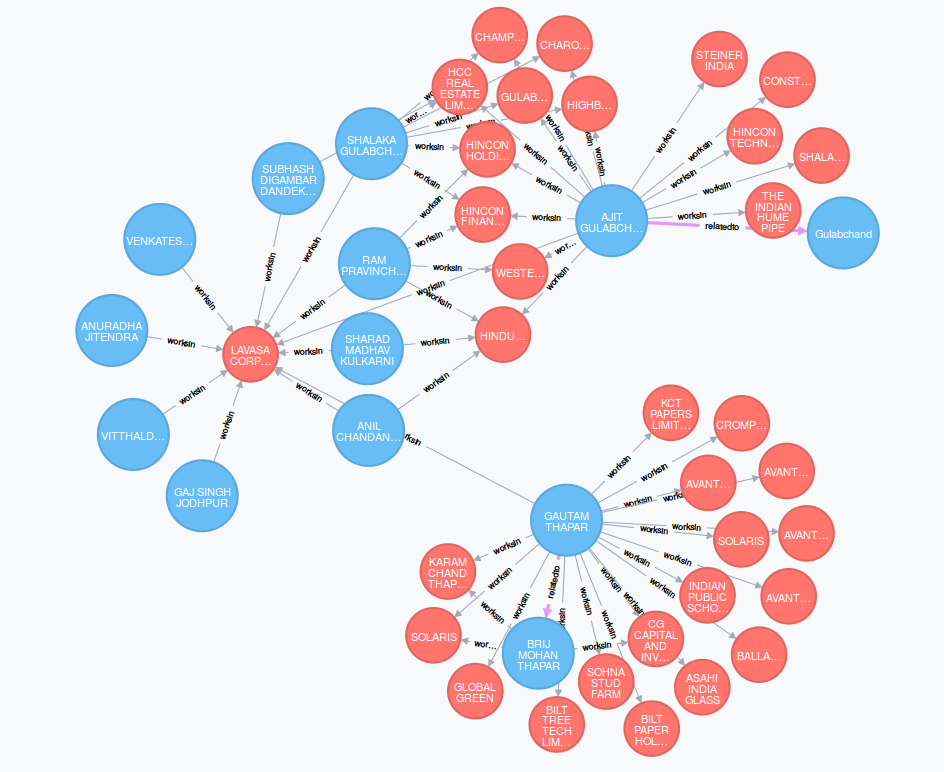
\includegraphics[width=1\textwidth]{lavasa} 
\caption{Gulabchands and Thapars}
\label{fig:lavasa}
\end{center}
\end{figure}


\section{Media Houses}

\subsection{Birlas, HT and Ambanis}

\begin{figure}[H]
\begin{center}  
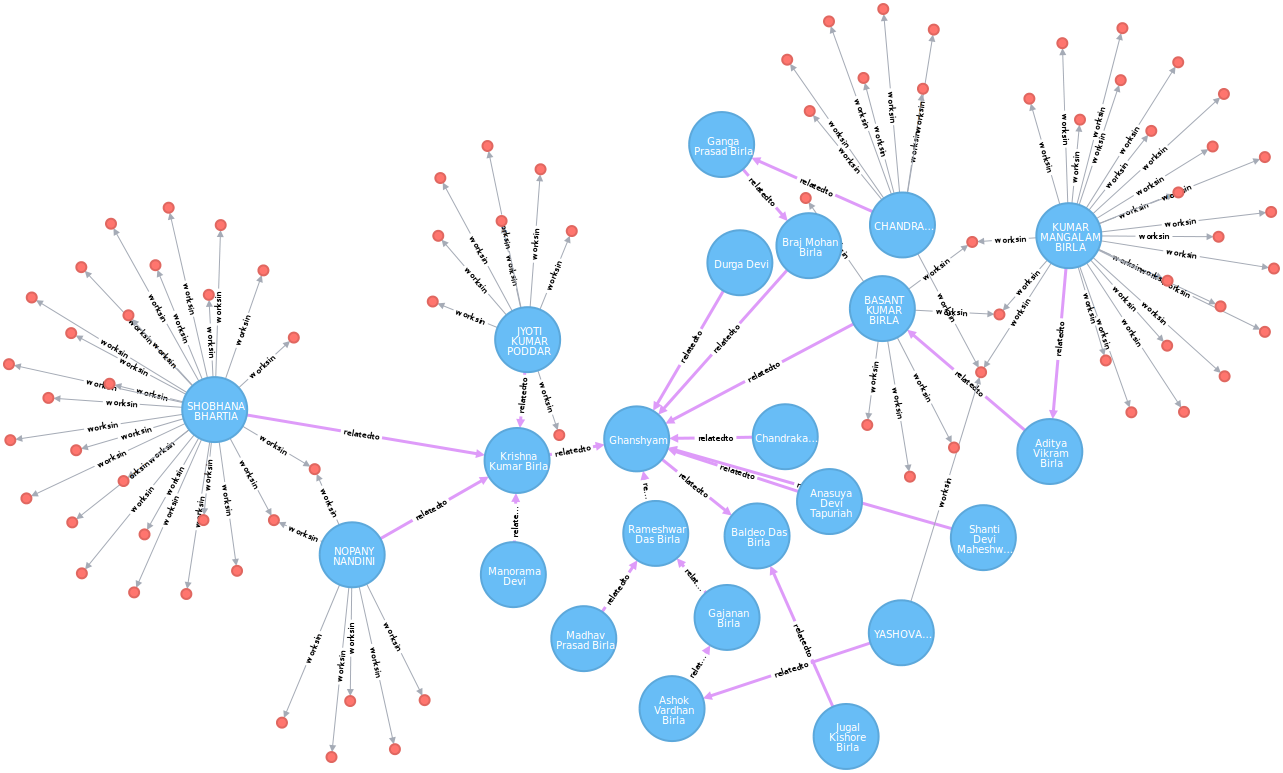
\includegraphics[width=1\textwidth]{ht} 
\caption{Shobhana Bhartia, Hindustan Times owner, ex-Rajya Sabha MP}
\label{fig:ht}
\end{center}
\end{figure}

\subsection{The Sarkars}

\begin{figure}[H]
\begin{center}  
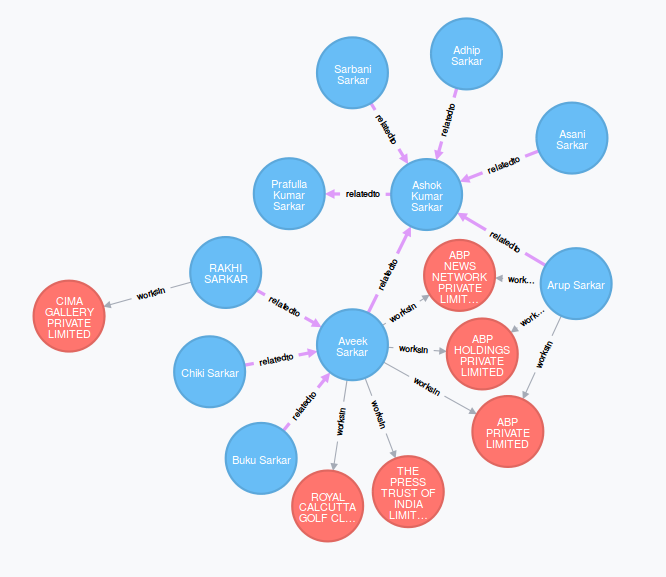
\includegraphics[width=1\textwidth]{sarkar} 
\caption{Aveek Sarkar of the Telegraph and ABP group}
\label{fig:sarkar}
\end{center}
\end{figure}


\section{Family trees}

\subsection{Ambani's}

\begin{figure}[H]
\begin{center}  
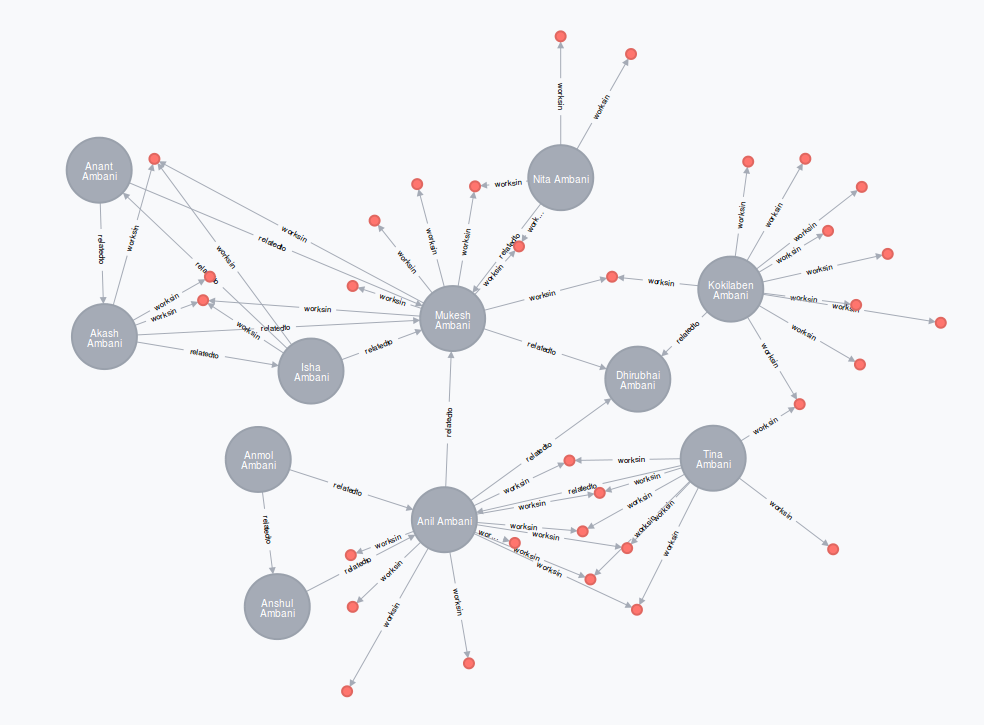
\includegraphics[width=1\textwidth]{ambani} 
\caption{Reliance: It's all in the family}
\label{fig:ambani}
\end{center}
\end{figure}


\subsection{The better halves}

\begin{figure}[H]
\begin{center}  
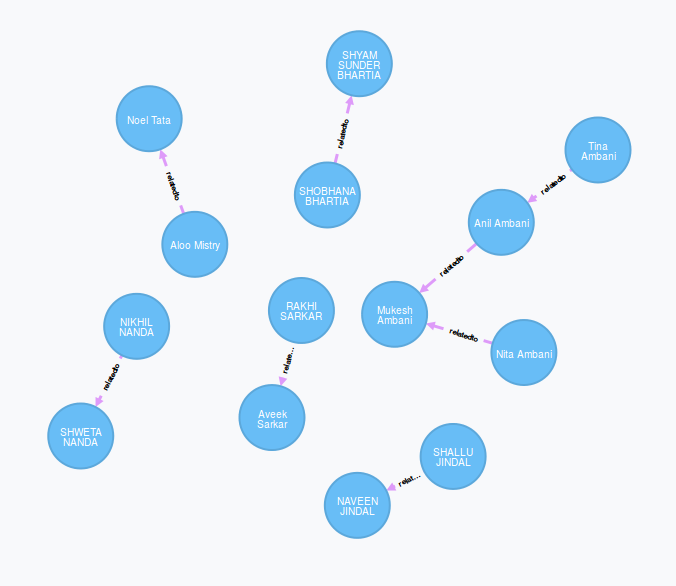
\includegraphics[width=0.8\textwidth]{spouses} 
\caption{Businesswomen and also spouses}
\label{fig:spouses}
\end{center}
\end{figure}


\subsection{Yadavs from UP and Bihar}

\begin{figure}[H]
\begin{center}  
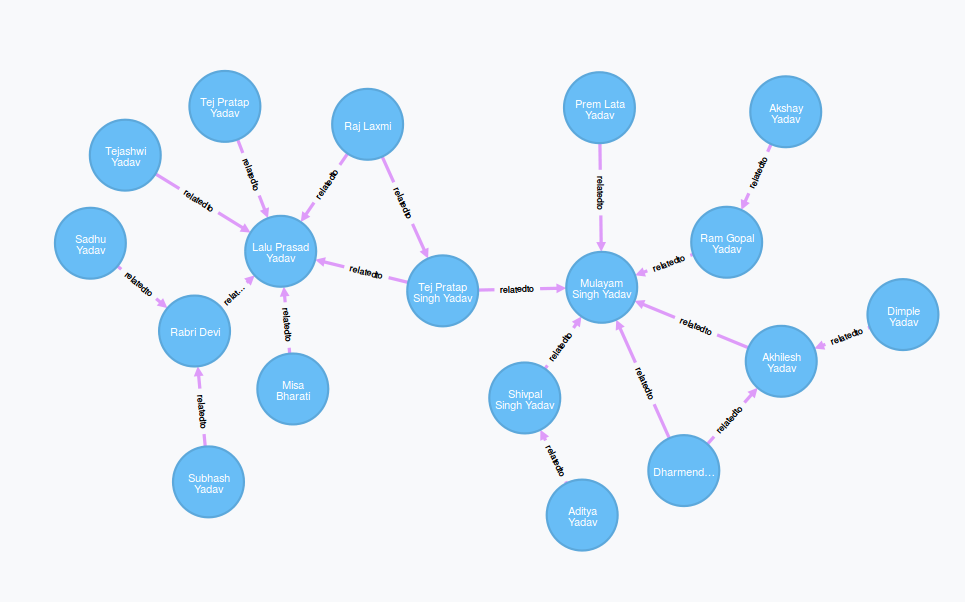
\includegraphics[width=0.8\textwidth]{yadavs} 
\caption{Connection between Lalu Prasad Yadav and Mulayam Singh Yadav}
\label{fig:yadavs}
\end{center}
\end{figure}


\section{Runaways or corporate hulks}

\subsection{Modis of Modinagar}

\begin{figure}[H]
\begin{center}  
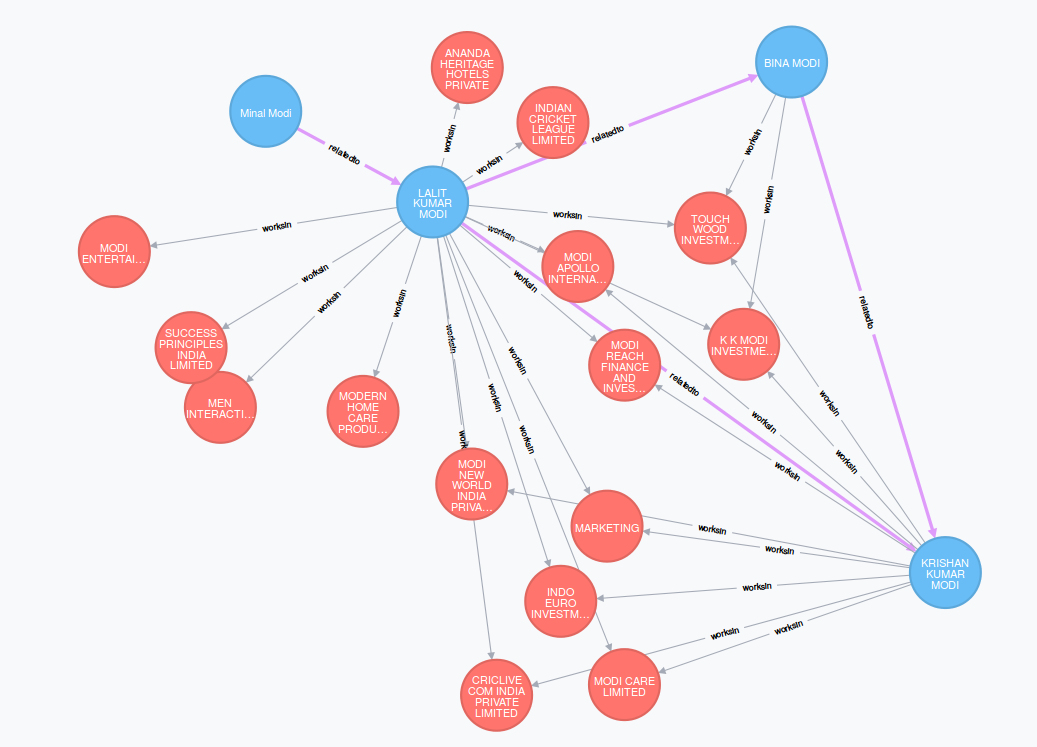
\includegraphics[width=1\textwidth]{modi} 
\caption{Lalit Modi of Modi dynasty}
\label{fig:modi}
\end{center}
\end{figure}


\subsection{Mallyas}

\begin{figure}[H]
\begin{center}  
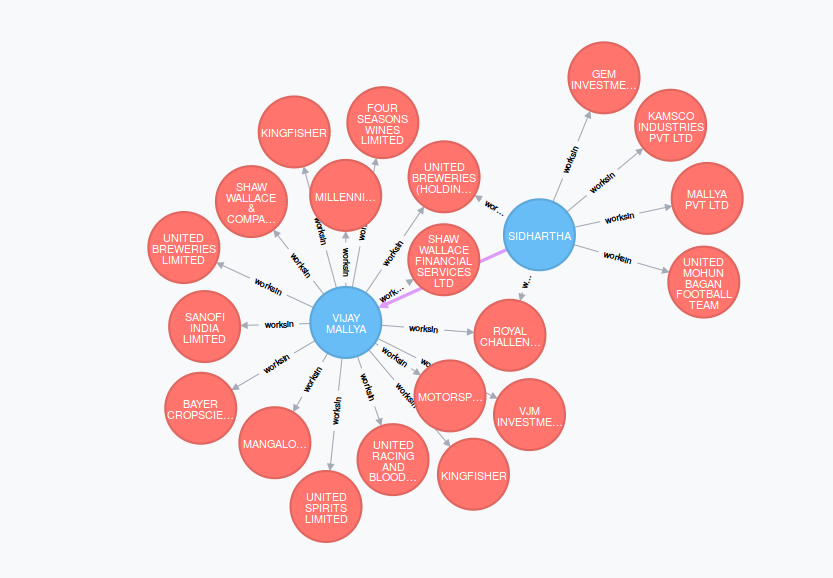
\includegraphics[width=1\textwidth]{mallya} 
\caption{Vijay mallya's empire}
\label{fig:mallya}
\end{center}
\end{figure}

\section{Arts, sports and commerce}

\subsection{Bachchans, Nandas, \& Kapoors}

\begin{figure}[H]
\begin{center}  
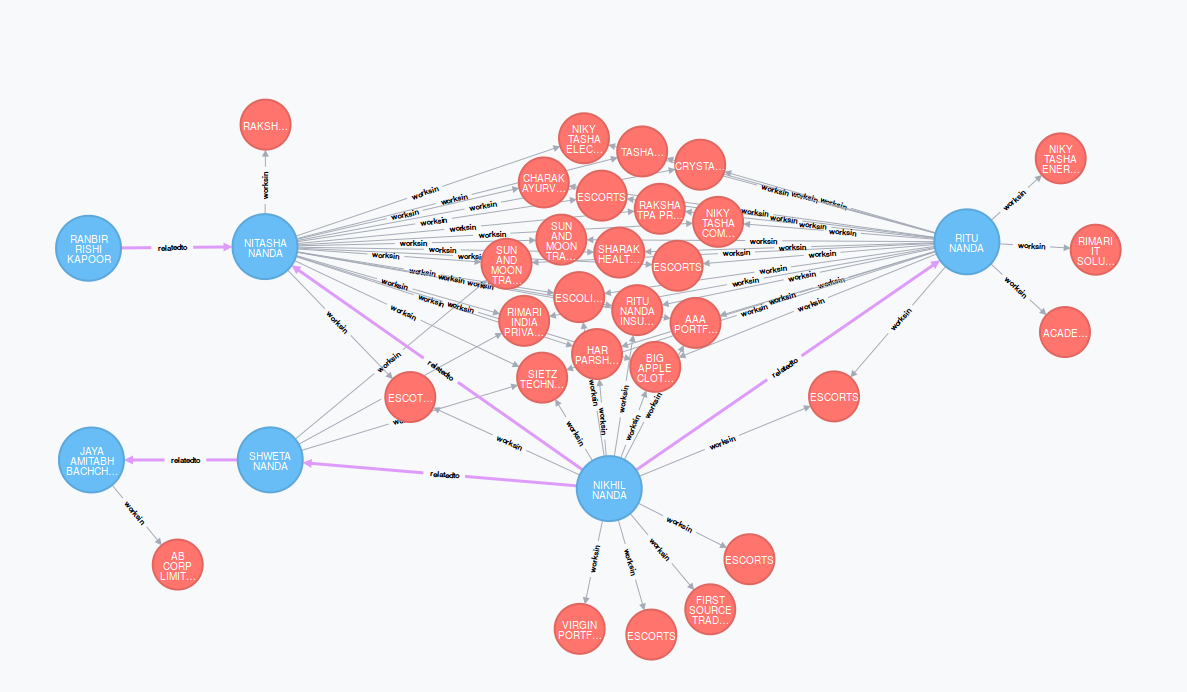
\includegraphics[width=1\textwidth]{nanda} 
\caption{One of the best examples of big houses marrying richer/bigger houses}
\label{fig:nanda}
\end{center}
\end{figure}

\subsection{King's XI Punjab and the boyfriend connection}

\begin{figure}[H]
\begin{center}  
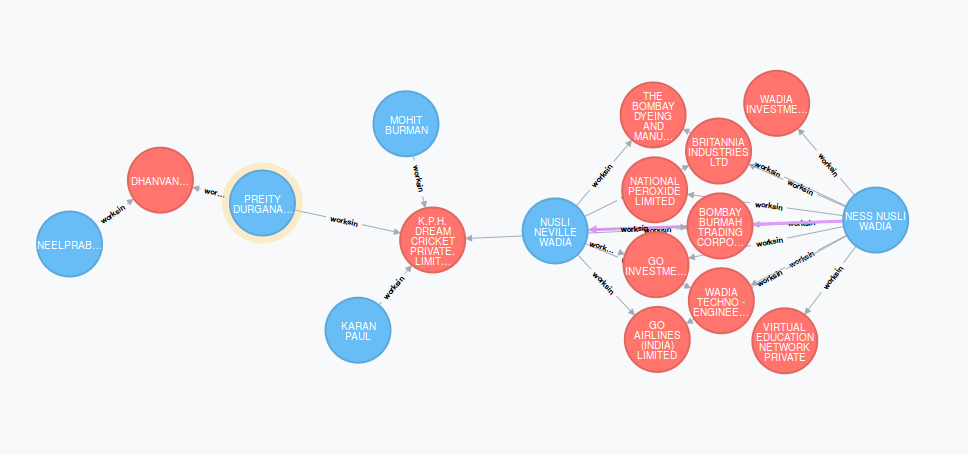
\includegraphics[width=1\textwidth]{wadia} 
\caption{Preity Zinta, holding a directorship in KXP, with the then-boyfriend Ness Wadia}
\label{fig:wadia}
\end{center}
\end{figure}

\subsection{Dada's family and business}

\begin{figure}[H]
\begin{center}  
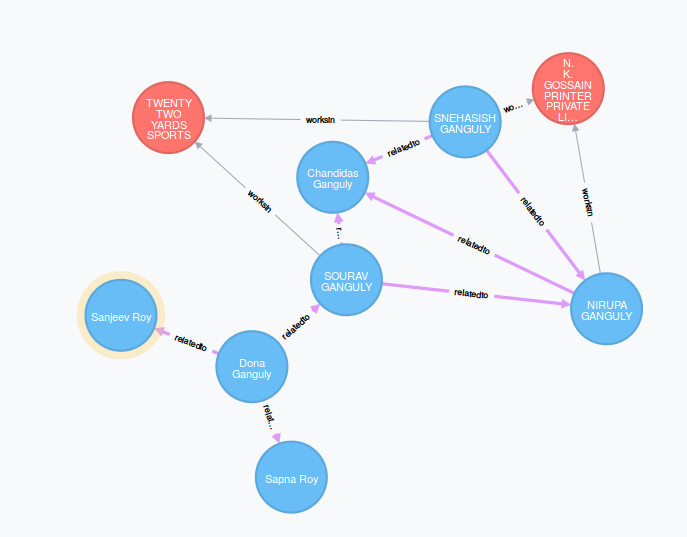
\includegraphics[width=1\textwidth]{ganguly} 
\caption{Sourav Ganguly and his company; his father is one the richest men in Kolkata}
\label{fig:ganguly}
\end{center}
\end{figure}



\section{Politics and Corporate}

There are numerous well known examples like Naveen Jindal and Jaydev Galla that recur time and gain in news. Here we mention some more.

\subsection{Gandhis and Vadra}

\begin{figure}[H]
\begin{center}  
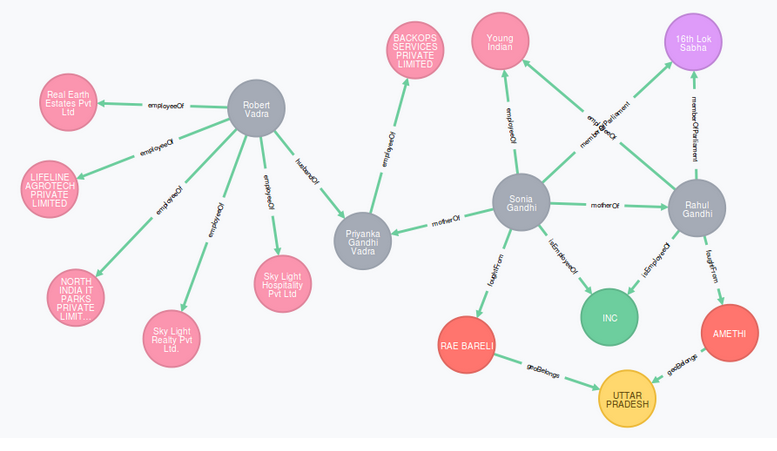
\includegraphics[width=1\textwidth]{gandhi} 
\caption{Gandhis and Son-in-law Vadra}
\label{fig:gandhi}
\end{center}
\end{figure}

\subsection{Jayant Sinha and his business-cum-political family}

\begin{figure}[H]
\begin{center}  
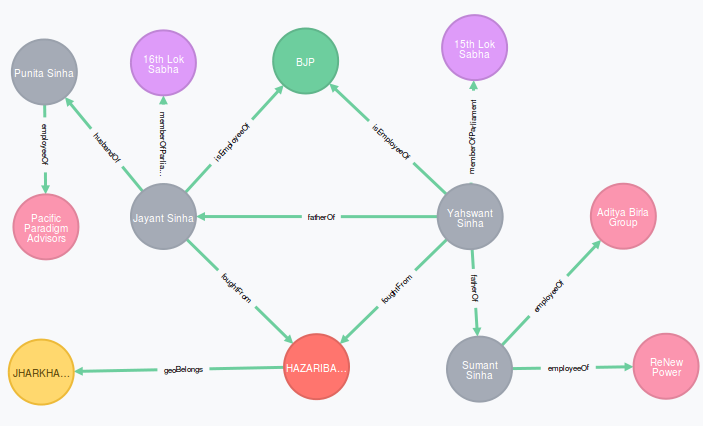
\includegraphics[width=1\textwidth]{sinha} 
\caption{Jayant Sinha and Family}
\label{fig:sinha}
\end{center}
\end{figure}

\subsection{Kamal Nath and Moser Baer}

\begin{figure}[H]
\begin{center}  
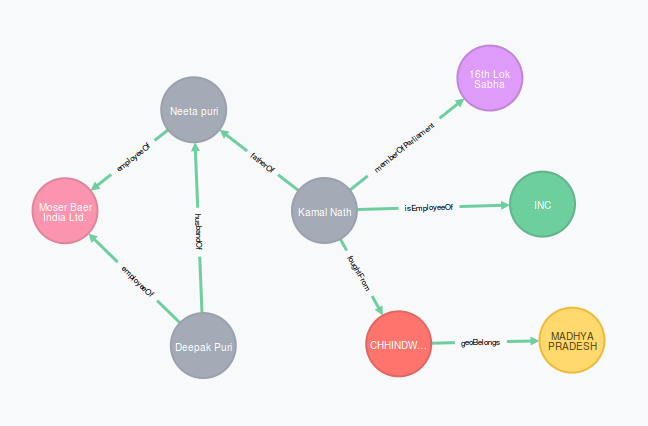
\includegraphics[width=1\textwidth]{nath} 
\caption{Kamal Nath and family}
\label{fig:nath}
\end{center}
\end{figure}